\documentclass{article}
\usepackage{amsmath, amssymb}
\usepackage{hyperref}
\usepackage{graphicx}
\usepackage{extarrows}
\title{Final Exam of Computational Neuroscience}
\author{Zhang Xiaorong\\ PB18061243}
\date{January 31,2021}
\begin{document}
\maketitle

\section*{Poisson Spike-Train Statistics}
\begin{enumerate}
    \item[1.]\begin{equation}
              \begin{split}
                  \langle n \rangle = \sum^\infty_{n=0} np(n) &= \sum^{\infty}_{n = 1}\dfrac{(rT)^n}{(n-1)!}\exp(-rT)\\
                  &=\exp(-rT)rT\sum_{n = 0}^\infty\dfrac{(rT)^n}{n!}\\
                  &=\exp(-rT) rT \exp(rT)\\
                  & = rT
              \end{split}
          \end{equation}
          \begin{equation}
              \begin{split}
                  \langle n^2 \rangle = \sum^\infty_{n=0} n^2p(n) &= rT \exp(-rT)\sum^{\infty}_{n = 0}\dfrac{(rT)^n}{n!}(n+1)\\
                  &=rT\exp(-rT)\left[\sum_{n = 0}^\infty n\dfrac{(rT)^n}{n!}+\sum_{n = 0}^\infty \dfrac{(rT)^n}{n!}\right]\\
                  &=rT\exp(-rT)\left[rT\exp(rT)+\exp(rT)\right]\\
                  & =(rT)^2+rT
              \end{split}
          \end{equation}
          \begin{equation}
              Var(n)= \langle n^2 \rangle-\langle n \rangle ^2= rT
          \end{equation}
          \begin{equation}
              Fano\ factor:\dfrac{Var(n)}{\langle n \rangle} = 1
          \end{equation}
          \begin{equation}
              \langle n^4 \rangle  = (rT)^4+6(rT)^3+7(rT)^2+rT
          \end{equation}
          \begin{equation}
              k =\langle n^4\rangle -3\langle n^2\rangle ^2 = -2(rT)^4+(rT)^2+rT
          \end{equation}
          if we replace $\langle n^4 \rangle $ with central moments, the result may look more beautiful:
          \begin{equation}
              \mu_4 = \langle (n-tT)^4 \rangle = 3(rT)^2+rT
          \end{equation}
          \begin{equation}
              k = \mu_4 - 3(rT)^2 = rT
          \end{equation}
    \item[2.]when it comes to inhomogeneous Poisson process:\\
          we devide time interval $[t_i,t_{i+1}]$ into M time bins of size $\Delta t$ and setting $M\Delta t = t_{i+1}-t_i$.
          we will ultimately take limit $\Delta t \rightarrow 0$. The firing rate during bin m within this interval is $r(t_i+m\Delta t)$,
          the firing probability of firing a spike in this bin is $r(t_i+m\Delta t)\Delta t$, the probability of not firing a spike is
          $1-r(t_i+m\Delta t)\Delta t$. So, to have no spike during the entire interval, we need string together the whole M bins,
          because the probability in each bin is independent, we just need to product them together.
          Denote entire spike numbers between initial time and time t $N(t)$
          \begin{equation}
              P[N(t_{i+1})-N(t_i) = 0] = \prod_{m=1}^M(1-r(t_i+m\Delta t)\Delta t)
          \end{equation}
          \begin{equation}
              \begin{split}
                  \ln P[N(t_{i+1})-N(t_i) = 0] &= \sum_{m=1}^M\ln(1-r(t_i+m\Delta t)\Delta t)\\
                  &\xlongequal{t\rightarrow 0}-\sum_{m = 1}^Mr(t_i+m\Delta t)\Delta t\\
                  &=-\int^{t_{i+1}}_{t_{i}}r(t)dt
              \end{split}
          \end{equation}
          the probability density $p(t_1,t_2,...,t_n)$ is the product of the densities for the individual
          spikes and the probabilities of not generating spikes during the interspike intervals,
          between time 0 and the first spike, and between the time of the last spike and the end of the trial period:
          \begin{equation}
              \begin{split}
                  &p(t_1,t_2,...,t_n) \\
                  =&P[N(t_1)-N(0) = 0]\cdot P[N(T)-N(t_n) = 0]\cdot\\
                  &\quad \prod_{i = 1}^{n-1}P[N(t_{i+1}-N(t_i)) = 0]\cdot\prod^{n}_{i = 1}r(t_i) \\
                  = &\exp\left(-\int_0^Tr(t)dt\right)\prod_{i=1}^{n}r(t_i)
              \end{split}
          \end{equation}
          \begin{equation}
              \begin{split}
                  &p[N(T)-N(0) = n]\\
                  =& \int_0^T dt_1 \cdots\int_0^Tdt_np(t_1,t_2,...,t_n)/n!\\
                  =& \exp\left(-\int_0^Tr(t)dt\right)\int_0^Tr(t_1)dt_1\cdots\int_0^Tr(t_n)dt_n/n!\\
                  =&\left(\int_0^Tr(t)dt\right)^n\exp\left(-\int_0^Tr(t)dt\right)/n!\\
                  &n=0,1,2\dots
              \end{split}
          \end{equation}
          it is very similar to homogeneous situation, when r(t) = r(const), this expression returns to homogeneous result
          \begin{equation}
              \langle n \rangle = \int_0^Tr(t)dt
          \end{equation}
          \begin{equation}
              Var(n) = \int_0^Tr(t)dt
          \end{equation}
          \begin{equation}
              Fano\ factor:\dfrac{Var(n)}{\langle n \rangle} = 1
          \end{equation}
          the result is the same as homogeneous's
    \item[3.]Reference the \textbf{poisson spike generator} on page 30 of therotical Neuroscience book.
          First, generate the interspike intervals from an exponential probability density. Then extend it to time-dependent rates by using
          rejection sampling. Rejection sampling requires a bound $r_{max}$ on the estimated firing rate such that $r_{est}(t) \leq r_{max}$ at all times.
          We first generate a spike sequence corresponding to the constant rate $r_{max}$
          by iterating the rule $t_{i+1} = t_i - \ln(x_{rand})/r_{max}$. The spikes are then thinned
          by generating another $x_{rand}$ for each i and removing the spike at time $t_i$
          from the train if $r_{est}(t_i)/r_{max} < x_{rand}$. If $r_{est}(t_i)/r_{max} \geq x_{rand}$, spike i is retained.
          Thinning corrects for the difference between the estimated time-dependent rate and the maximum rate.\\
          main code is in \texttt{poisson\_spike\_generator.m}.\\
          The following is 3 spike examples generated in 200 ms.\\
          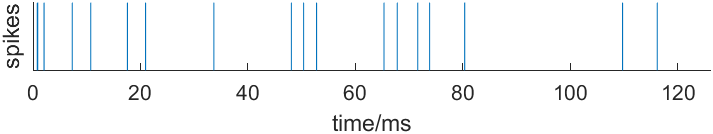
\includegraphics{pics/1_3_1.png}\\
          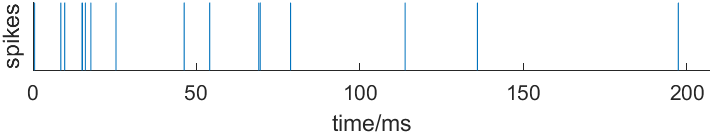
\includegraphics{pics/1_3_2.png}\\
          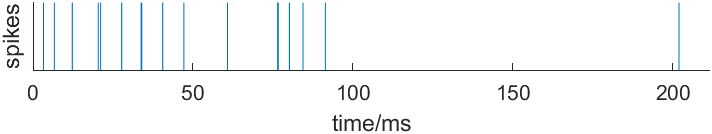
\includegraphics{pics/1_3_3.png}\\
          \\
          \\
          \\
          \\
          Next is a spike train in 20s:\\
          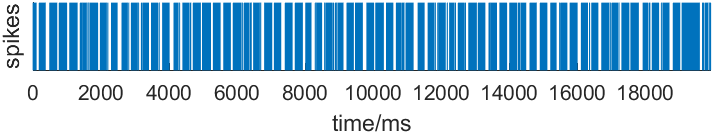
\includegraphics{pics/1_3_20s.png}
          Then, I did a mento carlo silmulation to test whether the sampling
          is right. Rerun the code I have used above s times, s is a large number,
          each s represents a trial. I roughly calculate r(t) using sampling result in a discrete way.
          r(ith time-bin)$\approx \langle n \rangle$, $\langle \rangle$ is mean from different trial, n is spike numbers in ith time-bin. i = 1,2,3\dots
          we could see from the following pic, the result is satisfactory, blue line is sample result,
          red line is real r(t), code is in \texttt{sample\_test.m}
          \\
          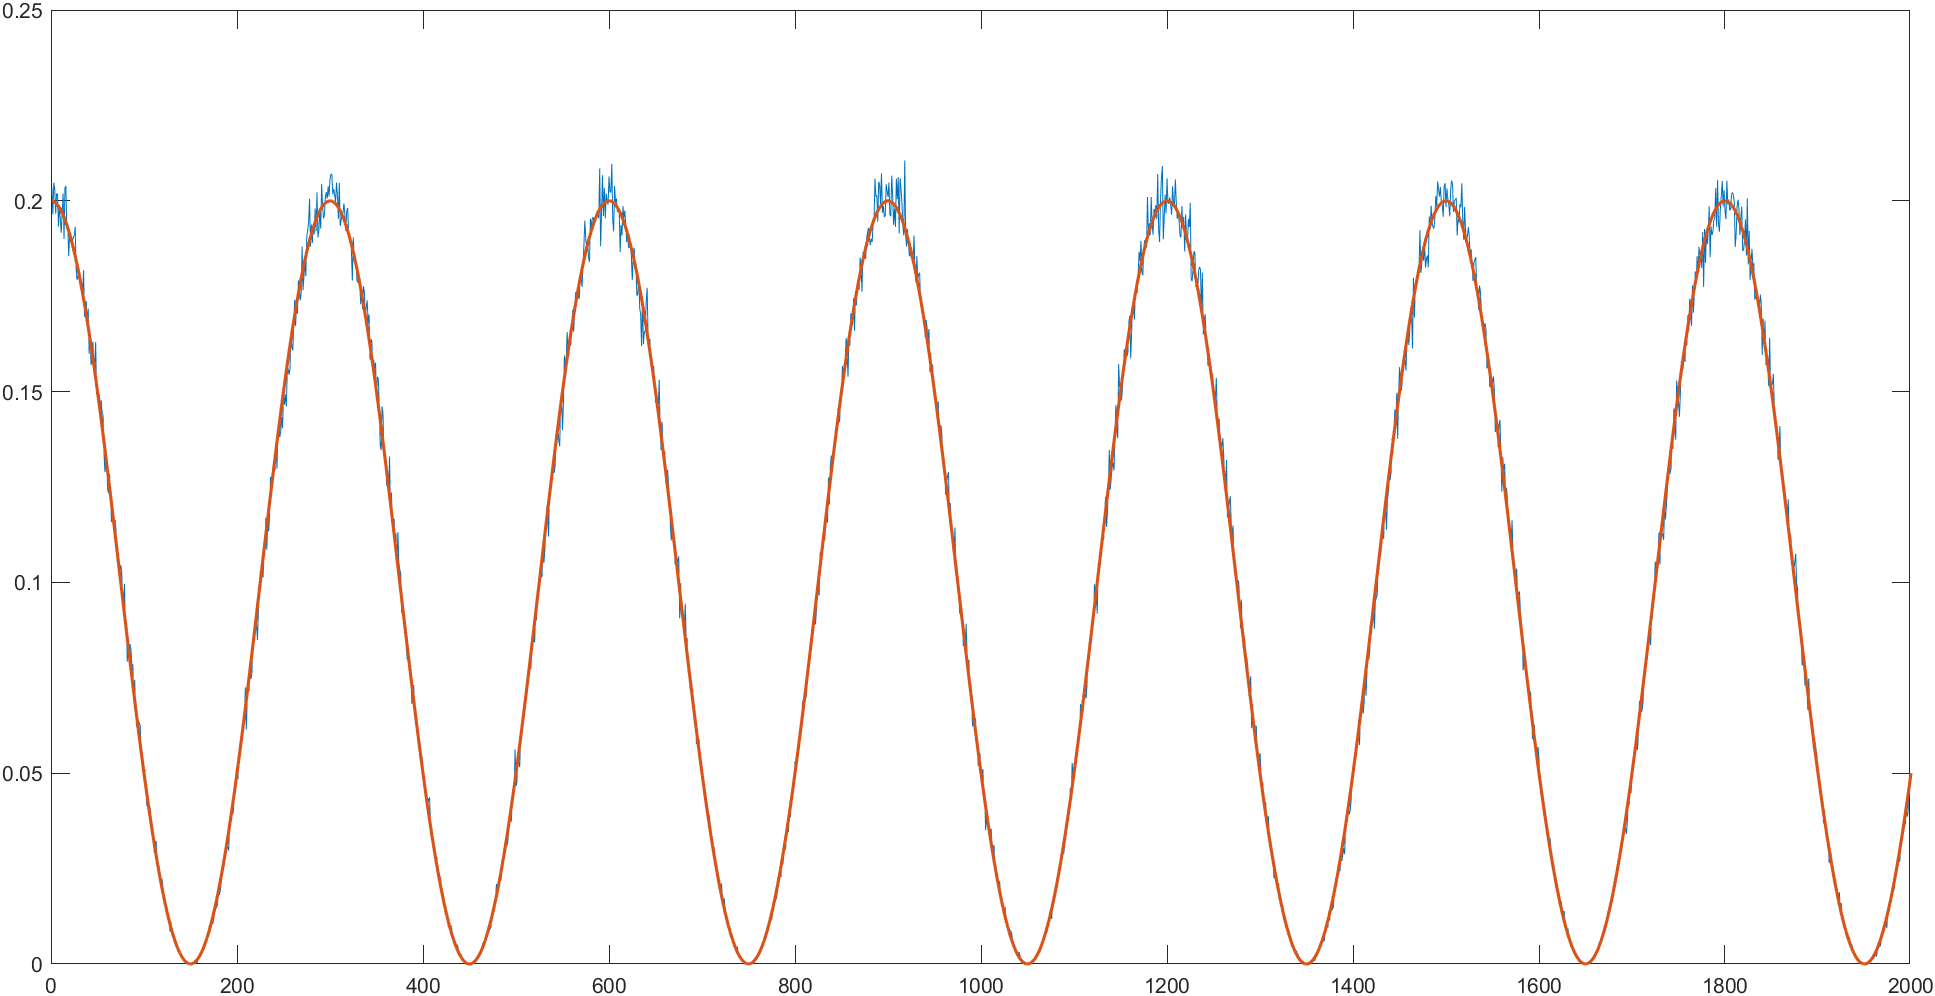
\includegraphics[scale = 0.35]{pics/r.png}

    \item[4.]In this problem, we need to use conditional expectation, use formula of total expectation twice
          \begin{equation}
              \begin{split}
                  \langle n \rangle &= E[E(n|\theta)] = E\left[\int_0^T(r_0+r_1 \sin(\omega t+\theta))d\right]\\
                  &=\dfrac{1}{2\pi}\int_0^{2\pi}d\theta\int_0^Tdt (r_0+r_1\sin(\omega t+\theta))\\
                  &= r_0 T
              \end{split}
          \end{equation}
          \begin{equation}
              \begin{split}
                  &\langle n^2 \rangle = E[E(n^2|\theta)]\\
                  &=\dfrac{1}{2\pi}\int_0^{2\pi}d\theta\left[\left(\int_0^Tr_0+r_1\sin(\omega t+\theta)dt\right)^2+
                      \int_0^Tr_0+r_1\sin(\omega t+\theta dt)\right]\\
                  & = (r_0 T)^2+\left(\dfrac{r_1}{w}\right)^2-\left(\dfrac{r_1}{w}\right)^2\cos\omega T+r_0 T
              \end{split}
          \end{equation}
          \begin{equation}
              \begin{split}
                  Var(n) = \langle n^2 \rangle - \langle n \rangle^2 = r_0T+2\left(\dfrac{r_1}{w}\sin\dfrac{\omega T}{2}\right)^2
              \end{split}
          \end{equation}
          \begin{equation}
              Fano\ factor:\dfrac{Var(n)}{\langle n \rangle} = 1+\dfrac{2\left(\dfrac{r_1}{w}\sin\dfrac{\omega T}{2}\right)^2}{r_0T}
          \end{equation}

\end{enumerate}

\section*{Sensory Neuron from an Electric Fish}
We consider times that are interger multiples of a basic unit of duration $\Delta t$,
that is times $t = m\Delta t$\ for m = 1,2,...,M where $M \Delta t = T$.
The function s(t) is then constructed as a discrete sequence of stimulus values.
This produce a steplike stimulus waveform, with a constant stimulus value $s_m$ presented during time bin $m$.
In terms of white-noise stimuli definition, each $s_m$ is uncorrelated means
\begin{equation}\label{def:white noise}
    \dfrac{1}{M}\sum_m^M \sum_n s_m s_n = \dfrac{\sigma_s^2}{\Delta t} \delta_{mn}
\end{equation}
where $\delta_{mn} = 0$,only if $m=n$
\begin{enumerate}
    \item[1.]When $t \in [(n-1)\Delta t,n \Delta t], s= s_n$,
          during each bin, the value of D could be seen as a constant,
          for example, when $t-\tau \in[(n-1)\Delta t,n\Delta t]$,$D(\tau)\approx D(t-n\Delta t)$.
          Then, we can replace integral with limited sum, the following eqaution could be obtained easily
          \begin{equation}
              \begin{split}
                  r(t) &= R_0+\int^\infty_0 D(\tau)s(t-\tau)d\tau\\
                  &= R_0+\sum_{n=-\infty}^{[t/\Delta t]} s_n D(t-n\Delta t)\Delta t \\
              \end{split}
          \end{equation}
          with the equation we have aquired above, we realize it in code \texttt{fish.m}. The stimulus and reaction is ploted in the following pictures\\
          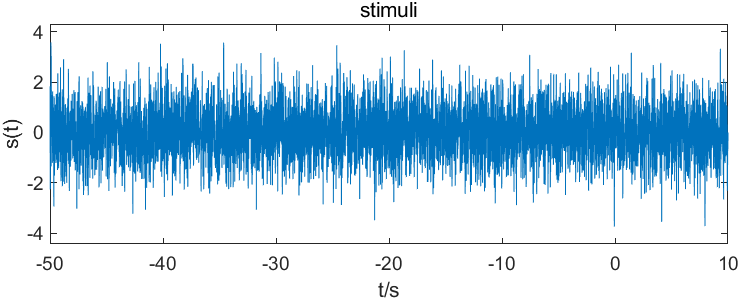
\includegraphics[scale = 0.8]{pics/2_1_stimuli.png}\\
          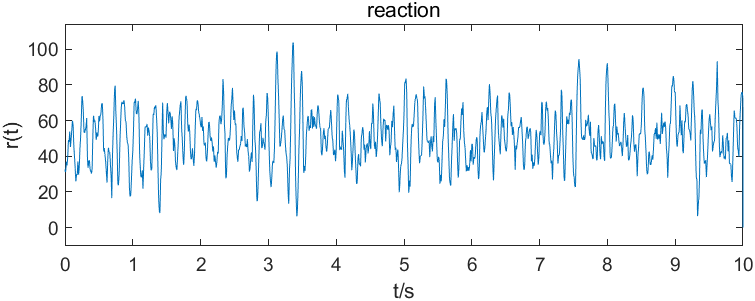
\includegraphics[scale = 0.8]{pics/2_1_reaction.png}

    \item[2.]
          Same as the previous question, replace the integral with limited sum, \\
          when $t+\tau \in[(m-1)\Delta t,m\Delta t]$,$D(t-n\Delta t)\approx D(m\Delta t-\tau-n\Delta t)$

          \begin{equation}
              \begin{split}\label{eqn:Qrs}
                  Q_{rs}(\tau) &= \dfrac{1}{T}\int^T_0 r(t)s(t+\tau)dt\\
                  &=\dfrac{1}{T}\int^T_0 (R_0+\sum_{n} s_n D(t-n\Delta t)\Delta t)s(t+\tau)dt\\
                  &= \dfrac{1}{T}\sum_m(R_0+\sum_{n} s_n D(m\Delta t -\tau-n\Delta t)\Delta t)s_m\Delta t\\
                  &= \dfrac{1}{T}\sum_m R_0 s_m(\Delta t)^2+\dfrac{\Delta t}{T}\sum_m \sum_n s_m s_n D[(m-n)\Delta t -\tau]\\
                  &=\dfrac{1}{M}\sum_m \sum_n s_m s_n D[(m-n)\Delta t -\tau]
              \end{split}
          \end{equation}
          omit $\dfrac{1}{T}\sum_m R_0 s_m(\Delta t)^2$ because it is higher order infinitesimal.
          Then, with the definition of white noise stimuli (\ref{def:white noise})
          \begin{equation}
              Q_{rs}(\tau) = \sigma_s^2 D[(m-n)\Delta t-\tau]\delta _{mn}=\sigma_s^2D(-\tau)
          \end{equation}
    \item[3.] From theoretical deduction, it is obvious that
          \begin{equation}
              Q_{rs}(-\tau)/\sigma^2 = D(\tau)
          \end{equation}
          The simulation result could be gotten from code \texttt{fish.m}
          In equation \ref{eqn:Qrs}, we omit the first term in forth line because when $\Delta t \rightarrow 0$, it is
          a higher order infinitesimal, but in my calculation, I replace integration with discrete sum, so
          $\Delta t$ is not infinitesimal, so when we compute $Q_{rs}$, if we minus $R_0$ from $R$, i.e. omit
          the first term manually, our result would be much more satisfactory.
          \\
          \\
          \\
          does not minus $R_0$:\\
          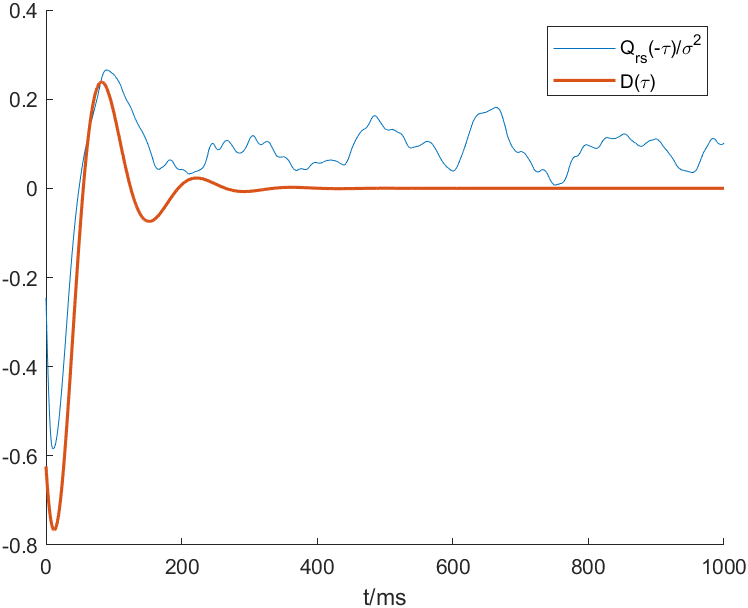
\includegraphics[scale = 0.8]{pics/Qrs1.png}

          minus $R_0$:\\
          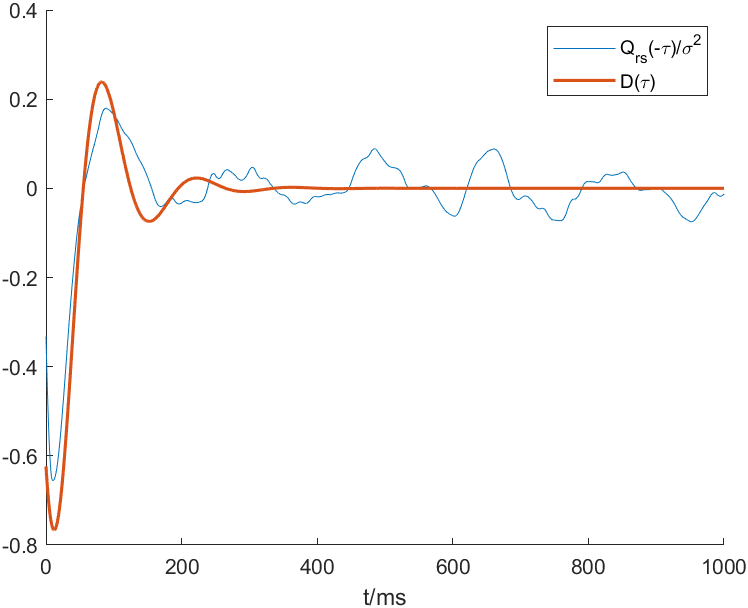
\includegraphics[scale = 0.8]{pics/Qrs2.png}
\end{enumerate}

\section*{Winner Take All Circuit}
\begin{enumerate}
    \item[1.]
          We have known the Lyapunov stability thereom, assume $x^*$ is equilibium point, the system is
          globally asymptorically stable if following conditions are satisfied
          \begin{itemize}
              \item $E(x^*) = 0$
              \item $E(x)>0,\forall x \neq x^*$
              \item $E(x)$ is radially unbounded
              \item $E(x)<0, \forall x\neq x^*$
          \end{itemize}
          the Lyapunov function is
          \begin{equation}
              E(x) =-\sum_{i}b_{i}x_{i}+\frac{1}{2}(1-\alpha )\sum_{i}x_{i}^{2}+\frac{%
                  \beta }{2}\sum_{i\not=j}x_{i}x_{j}
          \end{equation}
          Then,
          \begin{equation}
              \begin{split}
                  \dfrac{dE}{dt} &= \dfrac{dE}{dx}\dot{x} = \sum_i(-b_i+(1-\alpha)x_i+\frac{\beta}{2}\sum_{j\neq i}x_j)(-x_i+[b_i+(Wx)_i]_+)\\
                  & = -\sum_{i}(-x_i+b_i+(Wx)_i)(-x_i+[b_i+(Wx)_i]_+)
              \end{split}
          \end{equation}
          when $b_i+(Wx)_i>0$, $\dfrac{dE}{dt} = -\sum_{i}(-x_i+b_i+(Wx)_i)^2\leq 0$, the equality holds when x is at equilibium point\\
          when $b_i+(Wx)_i<0$,$\dfrac{dE}{dt} = \sum_{i}x_i(-x_i+b_i+(Wx)_i)$, the discussion about this situation is a little complicated\\
          let's consider a suitable linear transformation
          \begin{equation}\label{trans}
              y_i = b_i+\sum w_{ij}x_j
          \end{equation}
          then we could get that the following two equalities are equivalent
          \begin{equation}
              \begin{split}
                  \dot{y}+y = b+W[y]_+&\xLongleftrightarrow{y = Wx+b}Wx+b+W\dot{x} = b+W[b+Wx]_+\\
                  &\xLongleftrightarrow{W invertible} x+\dot{x} = [b+Wx]_+
              \end{split}
          \end{equation}
          then, E for y is
          \begin{equation}
              E = \frac{1}{2}\sum_{kj}F_k(\delta_{kj}-w_{kj})F_j-\sum_k b_kF_k
          \end{equation}
          where $F_i = [y_i]_+$
          write E in vector form, $E = \frac{1}{2}F^T(\mathbb{I}-W)F-b^TF$, E is lower bounded if
          $z^T(\mathbb{I}-W)z$ is copositive, i.e. $z^T(\mathbb{I}-W)z>0 \forall z \neq 0$ with $z_i\geq 0, \forall i$,
          so, when it comes to the exact W we have, for simplicity, let the size of W is $(n \times n)$:
          \begin{equation}
              \begin{pmatrix}
                  F_1 & F_2
              \end{pmatrix}
              \begin{pmatrix}
                  1-\alpha & \beta    \\
                  \beta    & 1-\alpha
              \end{pmatrix}
              \begin{pmatrix}
                  F_1 \\
                  F_2
              \end{pmatrix}
              = (1-\alpha)(F_1^2+F_2^2)+2\beta F_1 F_2>0
          \end{equation}
          since is inequality has to hold for any $x\geq 0$ (and$\beta>0$), it has to hold that
          \begin{equation}
              \begin{split}
                  1-\alpha>0, \\i.e. \quad \alpha <1
              \end{split}
          \end{equation}
    \item[2.]Reference the work we done in hw3 about the ring network, replace the \textbf{rectified linear network} with \textbf{x},
          then do calculation and analysis the result. \\
          First try to find the eigenvalue and eigenvector of W. let n = 3
          \begin{equation}
              \begin{vmatrix}
                  \alpha & -\beta & -\beta \\
                  -\beta & \alpha & -\beta \\
                  -\beta & -\beta & \alpha
              \end{vmatrix}
              \rightarrow
              \begin{vmatrix}
                  \alpha-2\beta & -\beta & -\beta \\
                  \alpha-2\beta & \alpha & -\beta \\
                  \alpha-2\beta & -\beta & \alpha
              \end{vmatrix}
              \rightarrow
              \begin{vmatrix}
                  \alpha-2\beta & -\beta       & -\beta       \\
                  0             & \alpha+\beta & 0            \\
                  0             & 0            & \alpha+\beta
              \end{vmatrix}
          \end{equation}
          it is easy to get the eigenvalues are $\{\alpha-(n-1)\beta,\alpha+\beta\}$,
          the eigenvector for $\alpha-(n-1)\beta$ is $(1,0,...,0)$,
          for $\alpha+\beta$ are unit vector in the other dimensions, eg. $e_i = (0,...,1,...,0),i = 2,3,...,n$\\
          let $x = \sum_k c_k e_k$, then the equation $\dot{x} = -x +[b+Wx]_+$ could be written as
          $$\sum_k\dfrac{dC_k}{dt}e_k = \sum_k c_k(\lambda_k-1)e_k+\overrightarrow{b}$$
          \begin{equation}
              \dfrac{dC_m}{dt} = C_m(\lambda_m-1)+\overrightarrow{b}\cdot e_m = C_m(\lambda_m-1)+b_m
          \end{equation}
          the solution is
          \begin{equation}
              c_m(t) = \dfrac{b_m}{1-\lambda_m}\{1-\exp[{-t(1-\lambda_m)}]\}+c_m(0)\exp(-t(1-\lambda_m))
          \end{equation}
          as same, let the exponent term do not explode, we request $\lambda_m < 1$, i.e.
          \begin{equation}
              \left\{
              \begin{aligned}
                  \alpha -(n-1)\beta<1 \\
                  \alpha +\beta<1
              \end{aligned}
              \right.
          \end{equation}
          but given that $\beta>1-\alpha$, i.e. $\alpha+\beta>1$, the second inequality cannot be satisfied,
          so when m = 2,3,...,n, the corresponding term will explode. Then, we replace \textbf{x} with \textbf{rectified linear network},
          the corresponding terms will converge to zero. \\
          Consider the leftover term ,\\
          $\alpha - (n-1)\beta<\alpha-(n-1)(1-\alpha) = 1+n*(\alpha-1)<1$\\
          so this term will converge to a steady state\\
          all in all, only a single neuron is active
    \item[3.]If just pick the neuron with largest $b_{max}$,
          when the system meets the steady state, $x_i^* = [b_i+(Wx)_i]_+ = b_i+\alpha x_i$,
          let $x_i = max_i b_i$, we could get $\alpha = 0$\\
          Further, consider the transformation \ref{trans} we have taken in the first question.
          if $x_j=0$ for all j except $j = argmax(b_j) = m$, this means $y_j = b_j +(Wx)_j = b_j-\beta b_m\leq 0, \forall j\neq m$,
          thus, $\beta\geq\dfrac{max_{j\neq m}b_j}{b_m}\rightarrow 1$\\
          all in all,
          \begin{equation}
              \alpha = 0,
              \beta = 1
          \end{equation}

          the following is some simulation results with code \texttt{winner\_take\_all.m}
          for simplicity, there are only 3 neurons, vector b is set to $\{4,5,0.5\}$. We can get
          more results by changing the initial conditions
          \\
          \\
          \\
          the situation in question 3, network picks the winner neuron:\\

          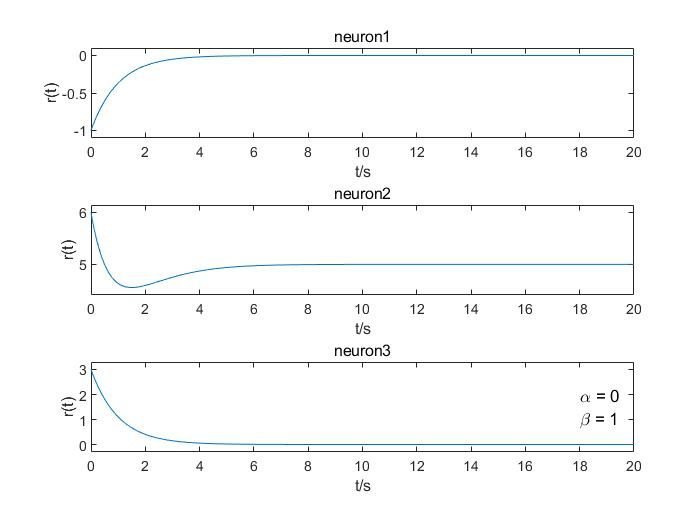
\includegraphics[scale = 0.55]{pics/3_1.jpg}
          \\
          \\
          \\
          \\
          \\
          not only one neuron is exited:\\
          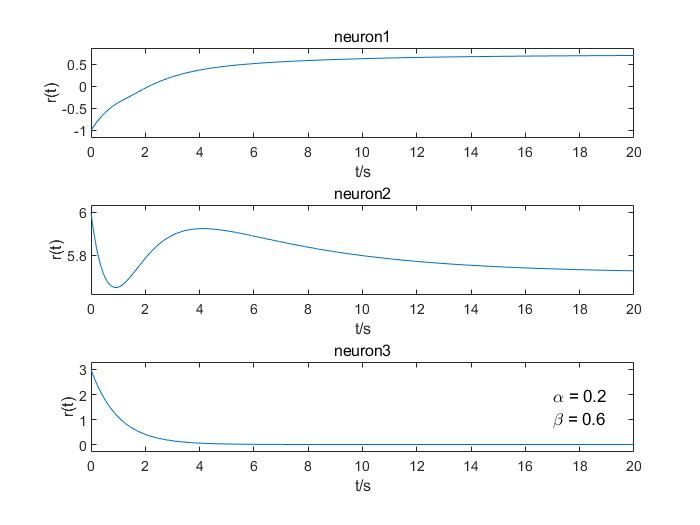
\includegraphics[scale = 0.45]{pics/3_2.jpg}
\end{enumerate}

\end{document}